\chapter{Úvod}
Zpracování řeči hraje v dnešní době důležitou roli v mnoha rozličných oborech. Mezi jedny z hlavních úkolů bezesporu patří separace zdrojů v nějakém zaznamenaném signálu, který může být složen ze signálů N mluvčích, ale i nechtěného hluku okolí. Vyřešení problému je předpoklad k dalším úkonům jako identifikace konkrétního mluvčího nebo třeba přepis nějaké konverzace na text. Se stále se zrychlujícím vývojem počítačů a s jejich zvyšujícím se výkonem se do popředí dostávají metody zpracování řeči založené na neuronových sítích, které v mnoha ohledech předčily doposud používané algoritmy.

Separace mluvčích v časové doméně dosahuje mimořádných výsledků v porovnání s dosavadními metodami LSTM založenými na převodu signálu z časové domény do frekvenční domény. Taková reprezentace signálu není optimální pro udržení časových závislostí, které jsou při zpracování řeči podstatné. V referenční studii je vstupní signál převeden do nezáporné reprezentace, která je optimální pro extrakci jednotlivých mluvčích. Silnou stránkou systému je hluboká architektura sítě, která lépe modeluje dlouhodobé závislosti v signálu.

Téma v oblasti neuronových sítí jsem si vybral, jelikož ty zažívají obrovský rozmach a pomalu se stávají součástí téměř všech odvětví a tudíž je velmi perspektivní pro další výzkum. Právě bakalářskou práci jsem vyhodnotil jako dobrou příležitost k seznámení se s neuronovými sítěmi a vyzkoušení si, jak se s nimi pracuje, jak se implementují modely za pomoci frameworku a jak náročná je aplikace na nějaký reálný problém.

\todo{spravit referenci na studii}
Mým úkolem v rámci práce je nastudovat si problematiku neuronových sítí a jejich základní principy, seznámit se problémem separace mluvčích pomocí neuronových sítí a následně implementovat síť podle architektury TasNet pro separaci mluvčích v časové doméně, která byla navržena a popsána ve studii \ref{referencni_studie}. Potom tuto neuronovou síť natrénovat s různými kombinacemi hodnot hyperparametrů, které ovlivňují velikost sítě a její vlastnosti, a nakonec porovnat přesnost a kvalitu separace mezi jednotlivými, různě velkými sitěmi a mezi výsledky studie. Přesnost separace je vypočítána pomocí míry si--snr, udávající poměr mezi chtěným signálem a hlukem na pozadí. Sítě budou testovány a vyhodnocovány na testovací množině jednokanálových směsí dvou mluvčích.

V první části práce, kterou pokrývá kapitola \ref{neuronovky}, jsou popsány základní prvky neuronových sítí, struktura umělého neuronu, jeho vstupy a výstupy, váhy a role aktivační funkce. V návaznosti na to je popsán proces učení neuronových sítí. Proces učení se skládá z několika souvisejících částí, které zahrnují výpočet výstupu neuronové sítě metodou feed forward, který transformuje vstupní vektor dat a počítá na základě něj výstupní vektor, který je předán zase další vrstvě a takto analogicky až do výstupní vrstvy. Dále je rozebrán výpočet chyby, která vzniká během procesu učení, metodou gradient descent a nakonec úprava vah neuronů metodou backpropagation (zpětná propagace chyby), která se počítá na základě rozdílu mezi vstupními hodnotami a očekávánými výstupními hodnotami.
\todo{Nejsem si jistej, jestli tohle je dobre s tim backprop atd, mam dojem ze backprop pocita gradienty, a ze obj funkce pocita chybu.}

Po vysvětlení základních principů je navázáno konvolučními neuronovými sítěmi, které jsou založeny na konvoluční operaci. Konvoluční sítě se používají nejčastěji pro zpracování obrazu kvůli vlastnostem, které umožňují extrahovat příznaky s různou úrovní složitosti od základních útvarů jako úsečka, barva a podobně až po komplexnější příznaky jako část obličeje -- ucho, nos, či úplně celý obličej. Tohoto lze využít i při zpracování zvuku, kde jsou tyto extrahované příznaky jednorozměrné.

Druhá část je věnována architektuře TasNet. V kapitole \ref{tasnet} je popsána podoba separačního modulu, jeho stavební bloky a princip. Postupně je zmíněn konvoluční auto-enkodér, u nějž je vysvětlen jeho úkol v separačním modulu a následně konvoluční blok, který se sám sestává z konvolučních vrstev, normalizací a aktivačních funkcí. Tyto bloky jsou skládány za sebe se zvyšující se časovou dilatací a tvoří jádro separačního modulu.

Kapitola \ref{implementace} se zabývá implementací neuronové sítě a jejím trénováním. Je popsána a zdůvodněna volba frameworku, implementace sítě a struktura zdrojového kódu. Pro usnadnění často se upakujících úkonů jsem vytvořil pár pomocných scriptů, které jsou zde také popsány. 
Model prošel během implementace několika úpravami. Pro účely trénování a validace byly vstupní nahrávky rozdělovány na čtyřsekundové segmenty. Pro testování byly používány nahrávky celé. V této kapitole je popsán průběh trénování sítí, výsledky a použité stroje a nástroje.

V poslední části, která je pokryta v kapitole \ref{experimenty} jsou shrnuty experimenty s modelem a vyhodnocení výsledků, v jehož rámci je zkoumán vliv hyper-parametrů na učení sítě, na výsledky a přesnost separace v závislosti na zvolených parametrech nebo počtu konvolučních bloků. Výstup sítě v podobě separovaných mluvčích je porovnán s referenční studií. Kvalita separace, neboli přesnost, je vypočítána pomocí si--snr metriky která udává poměr zastoupení chtěného signálu a hluku na pozadí. Je zde vyhodnoceno, jaký vliv má velikost sítě na přesnost separace a jsou zde shrnuty jednotlivé výsledky.

%----------------------------------------------------------------------------------------------------------------------------------------------------------------------
\chapter{Neuronové sítě}
\label{neuronovky}
V dnešní době zažívají neuronové sítě díky výkonosti počítačů velký rozmach. Jejich využití prostupuje skrze mnohé vědní obory a dokáží řešit celou řadu problémů, ve kterých dosahují výborných výsledků, které zdaleka předčily dosavadní postupy. 

Neuronové sítě jsou výpočetní model, který je inspirovaný strukturou lidského mozku, ve kterém je obrovské množství propojených a komunikujících neuronů. Ty se skládají ze vstupních dendridů, výstupních axonů a samotného těla neuronu. Na základě vnitřního potenciálu a vstupních hodnot je po přesažení prahové hodnoty vyslán signál na výstupní axon. Signál je nakonec předán dalším neuronům skrze jejich vstupní dendridy\cite[p.~65--66]{mitdeeplearning_small}.

Neurony v umělé neuronové síti jsou organizovány do vrstev, kde se každá vrstva může skládat z $1--N$ neuronů. První vrstva se nazývá vstupní, pak následují skryté vrstvy a nakonec výstupní vrstva.	

Účelem neuronové sítě je naučit se plnit zadanou úlohu. Rozdíl oproti běžným algoritmům je ale ten, že způsob, jakým síť má problém řešit, není explicitně naprogramován. Mezi problémy, které se dají řešit neuronovými sítěmi patří problémy v oblasti klasifikace, predikce a aproximace. Konkrétní příklad z oblasti klasifikace může být rozpoznávání objektů na obraze, psaného písma nebo detekce obličejů na videu, ale i mnohé aplikace ve zpracování řeči. Na základně řešeného problému vzniklo mnoho typů neuronových sítí, z nichž popsány budou konvoluční neuronové sítě. Začneme představením základního stavebního kamene -- neuronu.

\section{Umělý neuron}
Základní stavební jednotka neuronových sítí je neuron, nebo přesněji perceptron (viz obrázek \ref{fig:neuron}). Tento model je založen na principu reálných neuronů, které se nacházejí v organizmech. Perceptron obsahuje libovolně mnoho vstupních propojení, přes které se mu předávají data v podobě vstupního vektoru $\overrightarrow{x} = [x_1, x_2, \dots, x_n], x_n \in \mathbb{R}$. Sám neuron obsahuje hodnotu bias $b \in \mathbb{R}$ a vektor vah $\overrightarrow{w} = [w_1, w_2, \dots, w_n], w_n \in \mathbb{R}$, jehož modifikace představuje princip učení neuronu.

Výstupní hodnota závisí na vstupních datech, aktuálním vnitřním stavu (hodnoty vah a biase) a na zvolené aktivační funkci. Vstupní hodnoty jsou váhovány, což znamená, že každá vstupní hodnota je vynásobena s váhou na daném vstupním spojení, neboli, s použitím definovaných vektorů, lze napsat, že vstupní vektor je vynásoben s vektorem vah.

\begin{figure}[H]
    \centering
    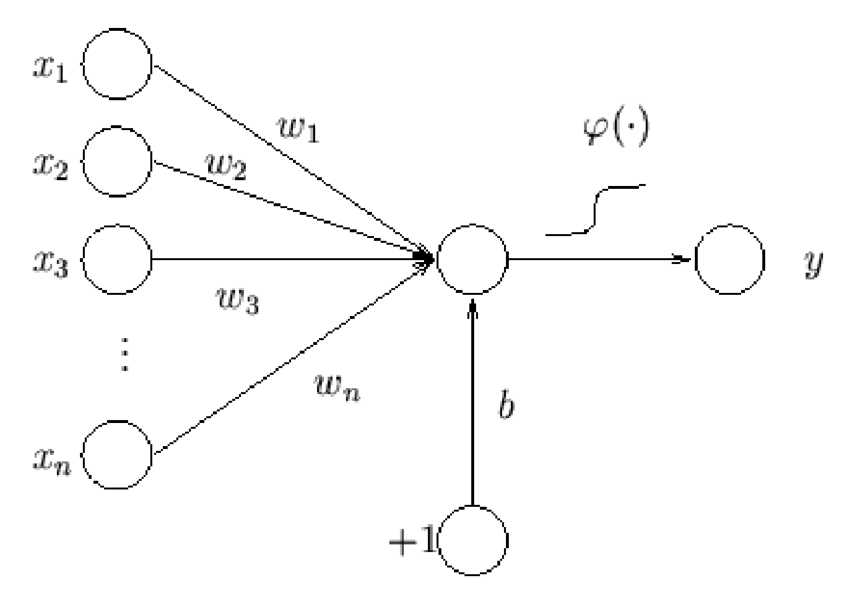
\includegraphics[scale=0.35]{obrazky-figures/perceptron.png}
    \caption{\label{fig:neuron}Schéma umělého neuronu -- perceptron}
\end{figure}

Hodnota bias $b$, která je přičtena k sumě násobků vah a vstupních hodnot, je prahová hodnota modifikující dobu, kdy se aktivuje perceptron a změní svůj výstup. Matematicky to znamená, že s grafem aktivační funkce horizontálně pohybuje doleva nebo doprava v závislosti na tom, je-li hodnota biasu pozitivní nebo negativní. Toto posunutí je znázorněno na obrázku \ref{fig:bias}. V závislosti na řešeném problému může být žádoucí, aby i hodnota bias byla modifikována během učení společně s ostatními váhami. V opačném případě je hodnota nastavena pevně na nějakou konstantní hodnotu, obvykle na jedna.

\begin{figure}[H]
    \centering
    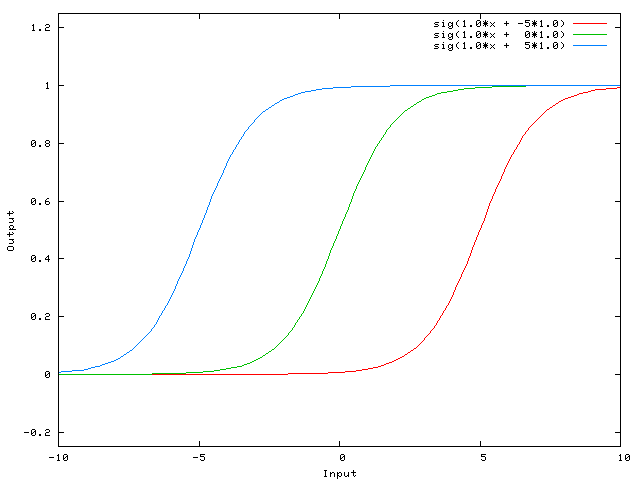
\includegraphics[scale=0.4]{obrazky-figures/bias.png}
    \caption{\label{fig:bias}Vliv hodnoty bias na aktivační funkci}
\end{figure}

Výstup neuronu se tedy vypočítá jako
\begin{equation}
y = f((\sum_{k=1}^n w_kx_k) + b)
\end{equation}
kde $f$ je nějaká aktivační funkce, $x_k \in \mathbb{R}$ je vstupní hodnota, $w_k \in \mathbb{R}$ je váha, kterou se vstupní hodnota vynásobí a $b \in \mathbb{R}$ je hodnota bias, která je přičtena k celkové sumě předtím, než je výsledek předán aktivační funkci.

\subsection{Aktivační funkce}
Aktivační, neboli prahová funkce určuje výstupní hodnotu neuronu. Funkce se vybírá na základě problému, který se má neuronová síť naučit řešit. Správná volba prahové funkce vede k lepší konvergenci učení sítě. Naopak špatná volba může vést ke stále větší odchylce od správného řešení -- může divergovat. Povaha problému může vyžadovat specifické vlastnosti aktivační funkce - lineární nebo nelineární -- sigmoidní a podobně. Pro nestandardní problémy je obvykle potřeba experimentálně zjistit, která funkce bude nejlépe vyhovovat danému problému. 

\subsection*{Sigmoid}
\begin{equation}
  f(x) = \frac{1}{1+\exp(-z)}
\end{equation}

\todo{popsat}

\begin{figure}[H]
    \centering
    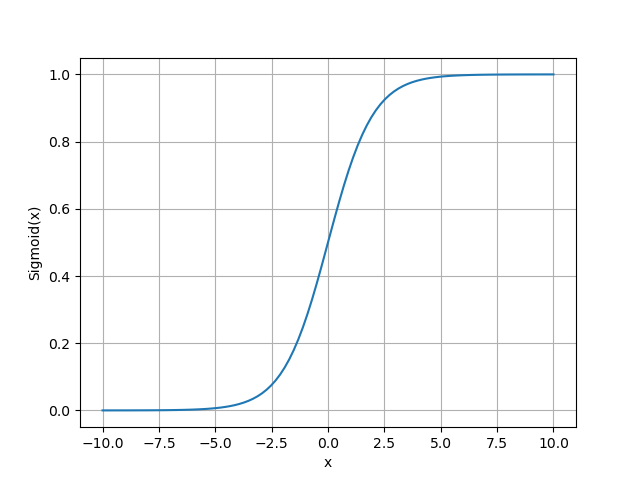
\includegraphics[scale=0.18]{obrazky-figures/sigmoid.png}
    \caption{\label{fig:sigmoid}Graf aktivační funkce sigmoid}
\end{figure}

\subsection*{Softmax}
\begin{equation}
  f(x) = \frac{1}{1+\exp(-z)}
\end{equation}

\todo{popsat}

\begin{figure}[H]
    \centering
    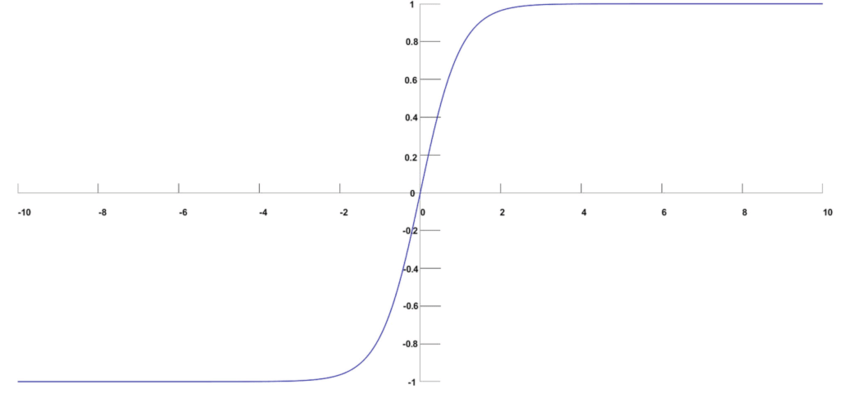
\includegraphics[scale=0.35]{obrazky-figures/softmax.png}
    \caption{\label{fig:softmax}Graf aktivační funkce softmax}
\end{figure}

Pokud by veškeré aktivační funkce v modelu byly lineární, tak celkové mapování sítě by bylo omezeno pouze na lineární mapování vstupu na výstup. Reálné problémy ale lineární obvykle nejsou a v případě pokusu modelovat takovým modelem nelineární vztahy by vedlo k velice nepřesným výsledkům, který by byl zapříčiněn podučením (underfitting), což znamená, že model, který se učí zakódovat nějaký vzor v datasetu, je příliš jednoduchý. Proto je potřeba zavést do modelu i nelineární aktivační funkce, které tento problém řeší\cite[p.~77--78]{mitdeeplearning_small}.

\subsection*{ReLU}
Rectified Linear Unit je nejčastěji používaná aktivační funkce. Vyžaduje-li neuronová síť nějakou nelinearitu, je ReLU pro většinu případů ideální. Pro každou zápornou hodnotu $x$ vrací $0$ a pro kladnou hodnotu $x$ vrací tutéž hodnotu $x$, jak udává rovnice 
\begin{equation}
   f(x)=max(0,x)
\end{equation}

\begin{figure}[H]
    \centering
    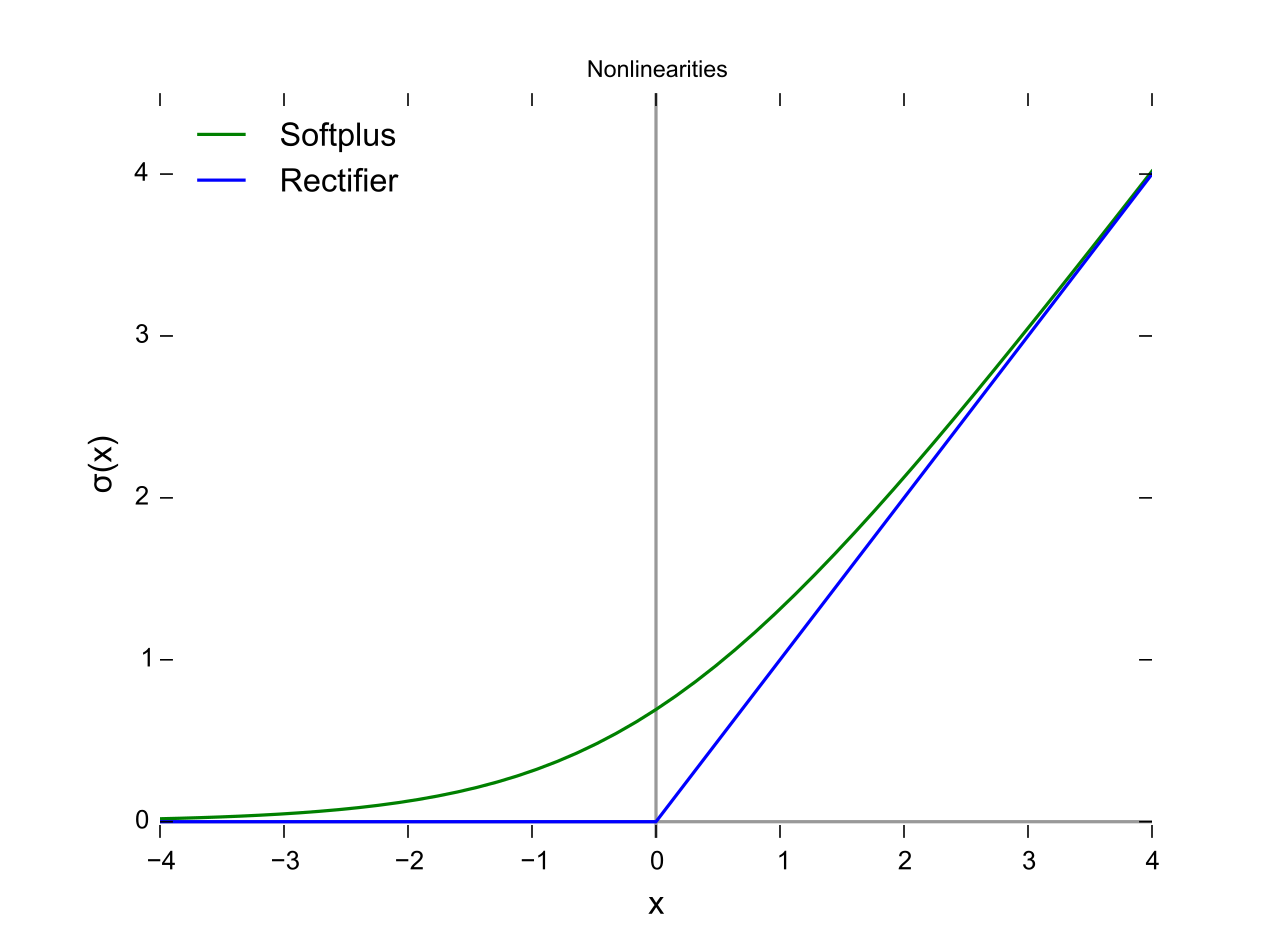
\includegraphics[scale=0.2]{obrazky-figures/ReLU.png}
    \caption{\label{fig:relu}Graf aktivační funkce ReLU}
\end{figure}


\subsection*{PReLU}
Parametrizovaná ReLU je nelineární aktivační funkce, která se používá v případě, že chceme produkovat na výstup malý nenulový gradient i v případě záporné vstupní hodnoty $x$. V tom případě je vstupní hodnota vynásobena parametrem $\alpha$ a to představuje výsledek. Parametr $\alpha$ se společně s ostatními váhami učí během učícího procesu.
\begin{equation}
  f(x) =
  \begin{cases}
    x & \text{if } x \geq 0 \\
    {\alpha}x & \text{if } x < 0
  \end{cases}
\end{equation}

\begin{figure}[H]
    \centering
    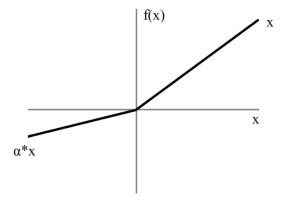
\includegraphics[scale=1.2]{obrazky-figures/prelu.jpg}
    \caption{\label{fig:prelu}Graf aktivační funkce PReLU}
\end{figure}

Jeden neuron však dokáže řešit klasifikaci pouze do 2 skupin a tím je pro složitější problémy nepoužitelný, ale propojením neuronů do vícevrstvé hierarchie lze řešit téměř libovolně komplexní problém. Takové seskupení se označuje jako vícevrstvý perceptron (Multi Layer Perceptron, MLP), neboli neuronová síť.

Nejzákladnější neuronová síť je tvořena třemi typy vrstev (viz obrázek \ref{fig:mlp}). Každá vrstva může obsahovat až $n, n \in \mathbb{N}/{0}$ neuronů. Vstupní vrstva slouží k předání hodnot do sítě, ale nijak tyto hodnoty nemodifikuje. Nezměněné jsou zkopírovány do první skryté vrstvy. Následují skryté vrstvy, z nichž poslední je napojena na výstupní vrstvu. Ta má obvykle méně neuronů než předešlé vrstvy a hodnoty na výstupu mohou představovat třídy, do kterých má být klasifikován vstup. S počtem jednotlivých vrstev souvisí pojem hloubka sítě, která je rovna počtu všech vrstev neuronové sítě od vstupní až po výstupní vrstvu. Pojmem hluboká neuronová síť se označuje taková síť, která má dvě nebo více skrytých vrstev.

Takto propojené neurony tvoří acyklický graf, který počítá a následně předává hodnoty směrem od vstupní vrstvy skrze skryté vrstvy až k vrstvě výstupní. Nenacházejí se zde žádná zpětná spojení, ve kterých by se výstup vracel zpět do sítě.\cite{mitdeeplearning}

\begin{figure}[H]
    \centering
    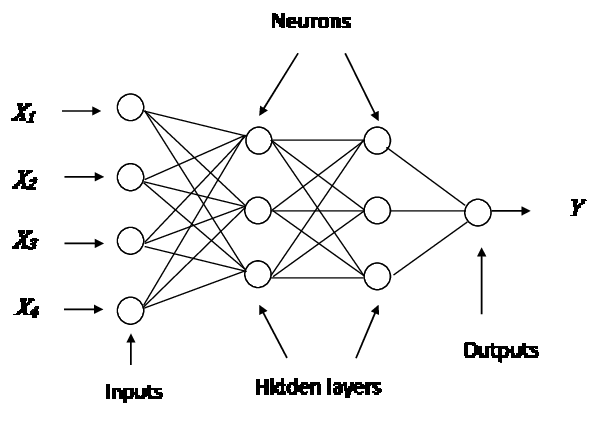
\includegraphics[scale=1.3]{obrazky-figures/mlp.png}
    \caption{\label{fig:mlp}Schéma neuronové sítě, která má 2 skryté vrstvy}
\end{figure}

Cílem takové neuronové sítě je aproximovat nějakou funkci $f^\ast$. Síti je předána vstupní hodnota $x$ a výstupní hodnota $y^\ast = f^\ast(x)$ má být co nejblíž hodnotě $y = f(x)$.






\section{Feed forward networks}
\todo{nepřejmenovat to na cz?}
\todo{v ramci tohoto proces uceni, cil uceni a objektivni funkce, MLP, }



\subsection{Objektivní funkce}
= cost funkce
-popis, co to je, k cemu to je, proc to je...

\subsection*{MSELoss}
- vzorecek
\subsection*{Cross Entrophy}
- vzorecek


\subsection{Optimalizační algoritmy}
 [1 deep learning str 301]

\subsection*{Adam}


Adam je jeden z algoritmů s adaptivním učením. Jeho název byl odvozen z fráze "adaptive moments".  [1 deep learning str 301]


\subsection{Backpropagation}
- zpetne sireni chyby
- adaptacni algoritmus, podil neuronu na chybe,
- 3 opakujici se faze uceni:

\todo{dodelat zde podkapitoly v lepsim poradi}

1) feedforward - dopredu
2) zpetne sireni chyby - Backpropagation
3) uprava vah a biasu na zaklade chyby
- chain rule



\subsection*{Gradient descent}

\subsection{Overfitting a generalizace}

\section{Konvoluční neuronové sítě}

\subsection{Konvoluce}


%----------------------------------------------------------------------------------------------------------------------------------------------------------------------


\chapter{TasNet - Time--Domain Audio Separation Network}
\label{tasnet}
\todo{Architektura full -- obrázek, bloky...}
\begin{figure}[H]
    \centering
    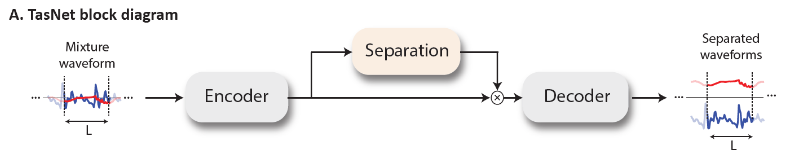
\includegraphics[scale=0.5]{obrazky-figures/tasnet-pipe.png}
    \caption{\label{fig:tasnet-pipe}Zjednodušený model architektury}
\end{figure}


\section{Konvoluční auto--enkodér}
\todo{Konvoluční autoenkodér, vstup, výstup...}

- schema bez separacniho modulu
- non negative representation of audio
\begin{figure}[H]
    \centering
    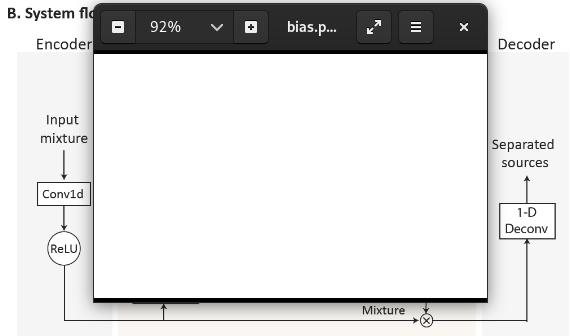
\includegraphics[scale=0.5]{obrazky-figures/tasnet-autoencoder.png}
    \caption{\label{fig:tasnet-autoencoder}Schéma konvolučního autoenkodéru}
\end{figure}


\section{Separační modul}
- odhad masek pro jednotlive mluvci
- schema se separacnim modulem
\begin{figure}[H]
    \centering
    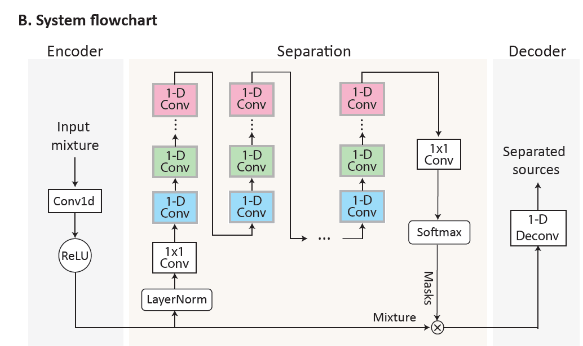
\includegraphics[scale=0.6]{obrazky-figures/tasnet-architecture.png}
    \caption{\label{fig:tasnet-modul}Schéma architektury TasNet}
\end{figure}


\subsection{Konvoluční bloky}
- Z čeho se skládá -- konvoluční vrstvy, normalizace
- diagram konv bloku.
- Mozna: Dilatace a time perception
\begin{figure}[H]
    \centering
    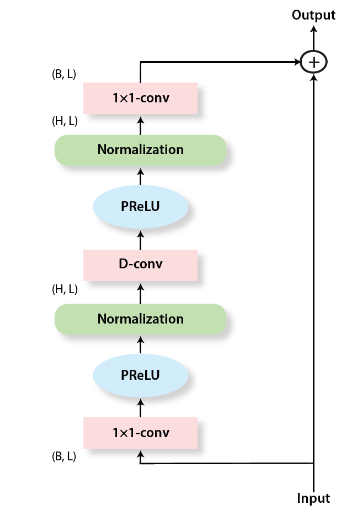
\includegraphics[scale=0.5]{obrazky-figures/conv-res-block.png}
    \caption{\label{fig:tasnet-convblock}Jeden konvoluční blok}
\end{figure}


%----------------------------------------------------------------------------------------------------------------------------------------------------------------------



\chapter{Implementace a trénování sítě}
\label{implementace}
Pozn: colab, pytorch, stroj, bash, hyperparams, vykon a cas trenovani, seg--len, popis trid.

\section{Implementace modelu}
- pytorch, scripty, python3, bash, tridy, moduly, parametry a volby spusteni.

\section{Dataset}
\todo{Ukazat zde vykreslenou vlnu nahravek mix, s1, s2}
\todo{popsat co je dataset a k cemu to slouzi}
Trénování a vyhodnocení modelu proběhlo na množině jednokanálových nahrávek směsí dvou mluvčích. Množina byla vygenerována náhodným výběrem různých mluvčích z Wall Street Journal (WSJ0) a vytvořením směsi. Celková délka trénovacích dat je přes 10 hodin a přes 6 hodin validačních dat. Nahrávky jsou převzorkovány na 8kHz a během trénování zarovnány na zero means a jednotkovou varianci[studie str 5 Dataset][49 - ze studie odkaz na script na generovani a popis na netu].
\begin{figure}[H]
    \centering
    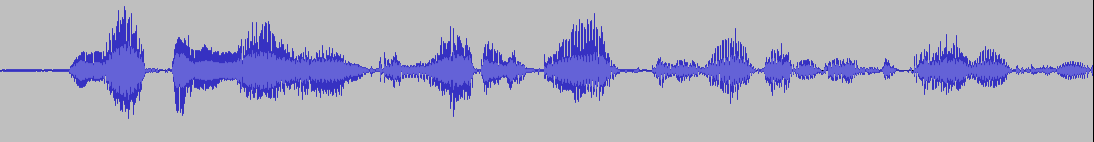
\includegraphics[scale=0.35]{obrazky-figures/dataset-mix.png}
    \caption{\label{fig:ref-mixture}Ukázka nahrávky směsi dvou mluvčích}
\end{figure}
\begin{figure}[H]
    \centering
    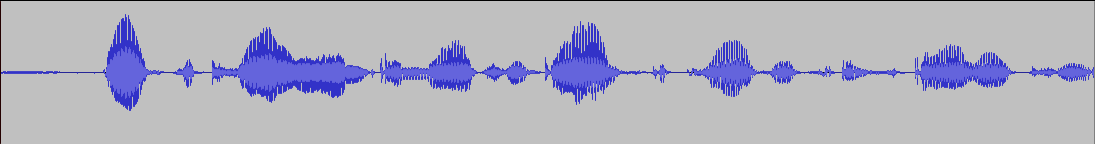
\includegraphics[scale=0.35]{obrazky-figures/dataset-s1.png}
    \caption{\label{fig:ref-s1}První mluvčí ze směsi}
\end{figure}
\begin{figure}[H]
    \centering
    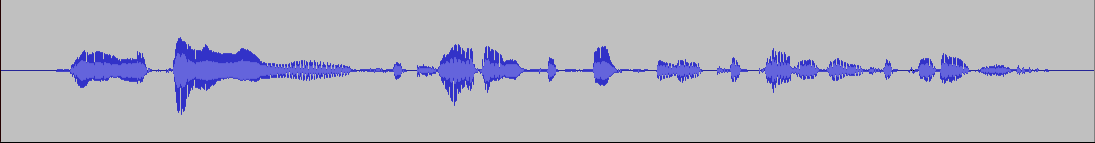
\includegraphics[scale=0.35]{obrazky-figures/dataset-s2.png}
    \caption{\label{fig:ref-s2}Druhý mluvčí ze směsi}
\end{figure}
Lze si všimnout, že sečtením signálů separovaných mluvčích na obrázku (ref obr1) a obrázku (ref obr2) dostaneme přesně signál směsi, což lze vyjádřit vztahem
\begin{equation}
  x(t) = \sum_{i=1}^C s_i(t)
\end{equation}
, kde $x(t) \in \mathbb{R}^{1 \times T}$ je diskrétní signál směsi a $s_i(t) \in \mathbb{R}^{1 \times T}$, kde $i = 1,\ldots,C$, je jeden z $C$ zdrojů[ref studie str3 vlevo]. 
\todo{doplnit info o zero means a jendotkove varianci}

\section{Trénování}
\begin{figure}[H]
    \centering
    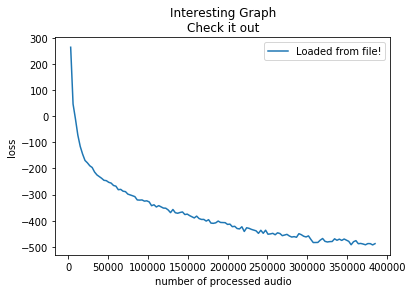
\includegraphics[scale=0.55]{obrazky-figures/some-loss.png}
    \caption{\label{fig:somelossTODO}Příklad grafu loss hodnoty během učení}
\end{figure}

\subsection{Význam validační množiny v trénování}
Většina algoritmů strojového učení má nějakou sadu hyperparametrů, kterou je upravováno chování algoritmu. Hodnoty hyperparametrů obvykle bývají nastavovány ručně ještě před spuštěním procesu učení a hodnota se v průběhu nemění, protože hodnoty by bylo obtížné optimalizovat. 
Některá nastavení se nicméně mohou stát hyperparametrem a být upravována během trénování, ale není vhodné je měnit na základě výsledku učení na trénovací sadě, protože by mohlo dojít k přetrénováníoverfitting) v důsledku \todo{CEHO??}. Pro tento případ potřebujeme validační sadu, která je odlišná od trénovací sady.
Po každém zpracování trénovací sady následuje validační sada, po jejímž skončení jsou optimalizovány hyperparametry[][].

\todo{[kniha 117-118] kap 5.3 = Hyperparameters and validation set} 
\todo{najit jeste nejakej zdroj s popisem a pripadne nejaky zajimavejsi info.}

\section{Vyhodnocovací metriky}
- minimalizovat objektivni-hodnotici funkci sisnr.
\subsection{Signal to noise ration}
\subsection*{Source Distortion Ratio -- SDR}
\subsection*{Artifacts Ratio -- SAR}
\subsection*{Inference Ratio -- SIR}



%----------------------------------------------------------------------------------------------------------------------------------------------------------------------


\chapter{Experimenty a vyhodnocení}
\label{experimenty}
- trenovani s ruznymi hyperparametry, uspesnost a tabulky s hyper parametry a dosazenymi vysledky a hodnotami sisnr, sdr atd.
- model size comparison.
- porovnani s vysledky ze studie
- obrazky separovanych mluvcich - signalu.
- spektra
- grafy trenovani loss a vysledkuu.
- pametova narocnost modelu


\section{Možná rozšíření a navrhnutá vylepšení}
- variabilnější dataset, mikrofony, šum a bordel prostředí
- separace více mluvčích
- hlučné prostředí
- identifikace konkrétního řečníka
- realtime separace

%----------------------------------------------------------------------------------------------------------------------------------------------------------------------

\chapter{Závěr}
\label{zaver}
- co jak dopadlo, vysledky a vyhodnoceni velikosti modelu a jaky byl nejlepsi,...

Cílem práce bylo implementovat síť podle architektury TasNet pro separaci mluvčích v časové doméně a porovnat vliv velikosti sítě na kvalitu separace. Síť byla implementována za pomoci frameworku pytorch a jazyku python a natrénována na datasetu obsahujícím jednokanálové směsi dvou mluvčích. Trénování proběhlo na \todo{X} modelech, které se od sebe lišily počtem opakujících se konvolučních bloků, velikostí časové dilatace a délkou vstupních segmentů směsí. Pro účel vyhodnocení modelů byla použita metrika si-snr, která udává poměr chtěného signálu ku šumu na pozadí, tedy obecně kvalitu separace. 

Experimenty ukázaly, že během testování nejlépe dopadla síť, která měla 8 konvolučních bloků po 4 opakováních, s délkou vstupního segmentu $L=2$ sekundy. Tento model dosáhl po 100 epochách trénování hodnoty až \todo{13,4} a tím se stal nejúspěšnějším modelem. Při fyzickém poslechu separovaných nahrávek bychom neslyšeli téměř žádný náznak druhého mluvčího. Oproti tomu, nejméně přesný model měl pouze 4 konvoluční bloky, 2 opakování a při délce segmentů $L=4$ sekundy dosahoval hodnoty SDR pouze \todo{9.2}.

Zkoušel jsem separovat také nahrávky, které byly úplně mimo dataset, ale výsledek se nedá hodnotit jako úspěšný, jelikož hraje velkou roli prostředí, mikrofon, šum v pozadí a další vlivy, na které byla neuronová síť naučena. Tento problém by se dal překonat rozšířením trénovacího datasetu o větší škálu nahrávek mluvčích, které by byly pořízeny z různých zařízení v různě rušném prostředí.

\TODO{Doplnit ještě neco?}



